\section{Introduction}
This paper uses \Cyclus, the agent-based simulator \cite{huff_fundamental_2016} to analyze
the future nuclear inventory in the European Union. This paper focuses on the spent fuel
inventory in \gls{EU} member states in 2050, and analyzes various potential strategies of spent fuel
management.
A major focus of this paper is to determine the extent to which France has an incentive
to receive all the \gls{SNF} from \gls{EU} nations to create \gls{MOX}.
The \gls{MOX} created will fuel French transition to a \gls{SFR} fleet
and may allow France to avoid building additional \glspl{LWR}.
A \Cyclus simulation is run to calculate
how much spent fuel is created from \gls{EU} nations from 1970 to 2050, as well as the amount
of \gls{MOX} that can be created with the \gls{SNF} inventory.
The paper assumes a once-through cycle for all 
\gls{EU} nations with the exception of France. France can reprocess spent \gls{UOX} and \gls{MOX} to
produce \gls{MOX} from reprocessed plutonium and depleted uranium (tails).
The simulation assumes \gls{MOX} is reprocessed infinitely. 
After obtaining the \gls{SNF} inventory of all \gls{EU} in 2050, a separate
simulation is run where the \gls{SNF} inventory is reprocessed and
used as fuel for the newly deployed \gls{SFR} reactors.
\gls{SFR} reactors in this paper models after the ASTRID reactor,
and use \gls{MOX} fuel created from 9\% reprocessed plutonium
and 91\% tailings to a burnup
of approximately 100 GWdth/t. The high burnup allows enough production of plutonium
for an equivalent mass of \gls{MOX}, if mixed with tailings.  Eventually,
the used \gls{UOX} inventory will be exhausted, and the \glspl{SFR} must be
fueled by \gls{MOX} created from recycled \gls{MOX}.
It is assumed that \glspl{SFR} are available for deployment
from 2040. 


\section{Methodology}
The work relies on \Cyclus, an agent-based simulator, to simulate the nuclear fuel cycle
and track material flows in \gls{EU} nations. The \gls{PRIS} open-source 
database from \gls{IAEA} was used to populate the simulation with deployment 
information. That database is imported as a csv file, listing the country, reactor unit, type, net capacity (MWe), status,
operator, construction date, first criticality date, first grid date, commercial date, shutdown
date (if applicable), and unit capacity factor for 2013. Then only the \gls{EU} countries are extracted
from the csv file. A python script is written up to generate a \Cyclus input file from the csv file,
which lists the individual reactor units as agents. After running the \Cyclus input file,
the output file is analyzed by another python script.

First, a simulation is run from 1970 to 2050 to calculate the mass of 
\gls{SNF} and depleted uranium (tails) \gls{EU} accumulates before 2050. 
The second simulation only looks at France, where France
uses the entire \gls{SNF} inventory from the previous
simulation to fuel
the newly deployed \glspl{SFR}. French \gls{SFR}s are deployed
to make up for the decommissioned capacity of \gls{LWR}s, to
remain a constant installed capacity of 60,000 MWe.

\subsection{Assumptions}
This paper makes the following assumptions:
\begin{itemize}
        \item \gls{SFR} technology available in 2040
        \item Decay has no effect on reprocessing viability
        \item Reactor construction is always completed on time 
        \item Unused separated uranium is stockpiled
        \item Nuclear power plants have a lifetime of 60 years, unless stated otherwise (early shutdown)
        \item (Only for SFR Case) French nuclear capacity remains constant at 60,000 MWe
        \item (Only for SFR Case) Infinite reprocessing and fabrication capacity
\end{itemize}


\subsection{Deployment Timeline}
Projections of future reactor deployment in this simulation were
assessed based on analysis from references like \gls{PRIS},
\cite{world_nuclear_association_nuclear_2017} \cite{joskow_future_2012} \cite{hatch_politics_2015}.
The projections extend to 2050 at the latest. This allows the simulation to take place from
1970 to 2050, the latest foreseeable future. The specific plans for each \gls{EU} nation are explained
in detail in later sections.

It is also assumed that all reactors that are 
currently operating have a lifetime of 60 years, unless their government plans
early shutdown. This will approximate when and how much \glspl{SFR} need to be built
to make up for the shutdown of \glspl{LWR}.

\subsection{French \gls{SFR} Deployment Schedule}

From 2040, when \gls{SFR}s become available,
600-MWe \gls{SFR}s are deployed to make up for the 
decommissioned \gls{LWR} capacities.

Initially in 2040, 22 \gls{SFR}s
are deployed for the previously decommissioned
\gls{LWR}s. From then, \glspl{SFR} are deployed to
make up for the decommissioned \gls{LWR} capacity.
This results in an installed capacity of 60,000 MWe
of \gls{SFR} by 2076.

\begin{figure}[htbp!]
        \begin{center}
                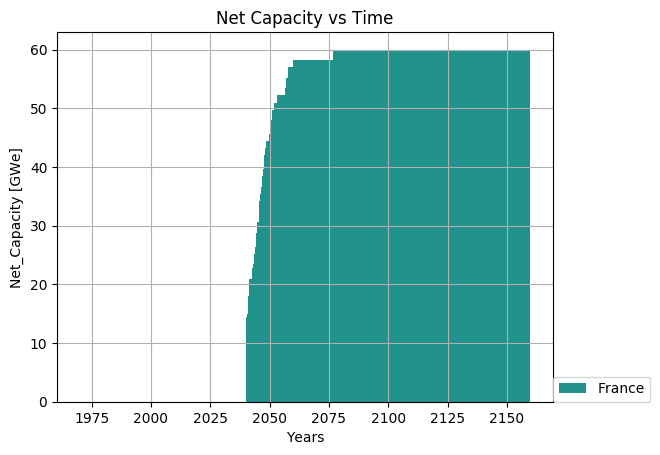
\includegraphics[scale=0.7]{./images/french-transition/power_plot.png}
        \end{center}
        \caption{Timeseries of installed capacity of \gls{SFR}s}
        \label{fig:sfr_cap}
\end{figure}


\begin{figure}[htbp!]
        \begin{center}
                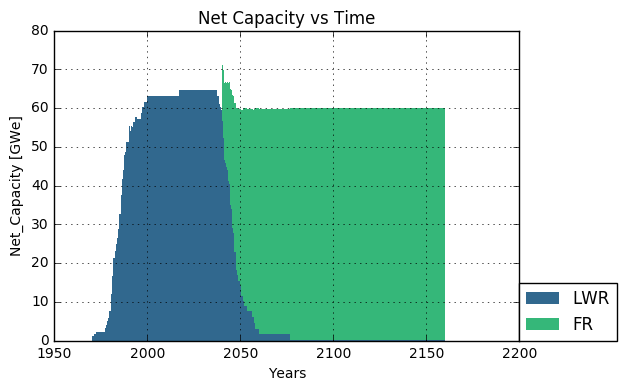
\includegraphics[scale=0.7]{./images/french-transition/number_plot.png}
        \end{center}
        \caption{Timeseries of number of \gls{SFR}s}
        \label{fig:sfr_num}
\end{figure}


Figures \ref{fig:sfr_cap} and \ref{fig:sfr_num}display
the \gls{SFR} number and capacity over time.
The sharp increase from 2035 to 2060 is due mainly to
French aggressive growth from 1975 to 2000.



\subsection{Depletion Calculations}
Depletion calculations of the nuclear fuel are recipe-based, such that a fresh 
and spent fuel recipe is used for each reactor type. To capture varying reactor 
capacity, a linear burnup model was assumed and extrapolated from the 
appropriate recipe. For example, a PWR of
1,000 MWe capacity has 193 assemblies of 3.2\% enriched
uranium fuel, with each assembly with a mass of 523.4 kg.
The core has a 18 month cycle, where one-third of the 
core (64 assemblies) are discharged per refueling. The refueling
is assumed to take 2 months to complete, during which the reactor
is shut down. For the \gls{SFR}, a model design is adopted from
Marsault–Marie-Sophie et al. \cite{marsaultmarie-sophie_pre-conceptual_2012}.

For the compositions of the fuel, a reference depletion calculation
from ORIGEN is used (see appendix). The recipe has also been used for
\cite{wilson_adoption_2009}.

\subsection{Scenario Descriptions}
The simulation follows the model fuel cycle, where a `source'
provides natural uranium, which is enriched by an 'enrichment'
facility to \gls{UOX}, while disposing enrichment waste (tailings)
to the 'sink' facility. The enriched \gls{UOX} is used
in the \gls{LWR}s and \gls{UOX} waste is produced. The spent fuel
is then reprocessed to separate plutonium and uranium.
The plutonium is mixed with depleted uranium (tails) to \gls{MOX}.
The reprocessed uranium is stockpiled. \gls{SNF} decay is assumed
to have no effect on reprocessing viability.


% Define block styles
\tikzstyle{decision} = [diamond, draw, fill=blue!20, 
text width=4.5em, text badly centered, node distance=3cm, inner sep=0pt]
\tikzstyle{block} = [rectangle, draw, fill=blue!20, 
text width=5em, text centered, rounded corners, minimum height=4em]
\tikzstyle{line} = [draw, -latex']
\tikzstyle{cloud} = [draw, ellipse,fill=red!20, node distance=3cm,
minimum height=2em]


\begin{figure}
        \centering
        \scalebox{0.8}{
                \begin{tikzpicture}[align=center, node distance = 3cm and 3cm, auto]
                % Place nodes
                \node [block] (sr) {Source};
                \node [cloud, below of=sr] (nu) {Nat U};
                \node [block, below of=nu] (enr) {Enrichment};
                \node [cloud, below of=enr] (uox) {\gls{UOX}};
                \node [block, below of=uox] (lwr) {\gls{LWR}};
                \node [cloud, right of=uox] (snf2) {\gls{SNF}};
                \node [cloud, left of=lwr] (tl2) {Tailings};
                \node [cloud, right of=enr] (tl) {Tailings};
                \node [block, right of=tl] (sk) {Sink};
                \node [cloud, below of=lwr] (snf) {\gls{SNF}};
                \node [block, below of=snf] (rep) {Reprocessing (Separations)};
                \node [cloud, below of=rep] (u) {Sep. U} ;
                \node [cloud, left of=rep] (pu) {Sep. Pu};
                \node [block, left of=pu] (mix) {Mixer (Fabrication)};
                \node [cloud, below of=mix] (mox) {\gls{MOX}};
                \node [block, below of=mox] (mxr) {\gls{MOX} Reactors};
                \node [cloud, right of= mxr] (snmox) {Spent \gls{MOX}};
                
                
                \draw[->, thick] (sr) -- (nu);
                \draw[->, thick] (nu) -- (enr);
                \draw[->, thick] (enr) -- (tl);
                \draw[->, thick] (enr) -- (tl2);
                \draw[->, thick] (tl) -- (sk);
                \draw[->, thick] (tl2) -- (mix);
                \draw[->, thick] (enr) -- (uox);
                \draw[->, thick] (uox) -- (lwr);
                \draw[->, thick] (lwr) -- (snf);
                \draw[->, thick] (lwr) -- (snf2);
                \draw[->, thick] (snf2) -- (sk);
                \draw[->, thick] (snf) -- (rep);
                \draw[->, thick] (rep) -- (u);
                \draw[->, thick] (rep) -- (pu);
                \draw[->, thick] (pu) -- (mix);
                \draw[->, thick] (mix) -- (mox);
                \draw[->, thick] (mox) -- (mxr);
                \draw[->, thick] (mxr) -- (snmox);
                \draw[->, thick] (snmox) -- (rep);
                
                \end{tikzpicture}
        
                }
                \caption{Model Fuel Cycle with \gls{MOX} Reprocessing}
                \label{diag:fc}
\end{figure}


The second scenario estimates the \gls{SNF} inventory in \gls{EU} at 2050,
and reprocesses the \gls{SNF} to separate plutonium. The separated
plutonium is mixed with the depleted uranium inventory from 2050
to create \gls{MOX}, which is used in the \gls{SFR}s. The used
\gls{MOX} is also reprocessed to extract plutonium, which also
is mixed with depleted uranium to produce \gls{MOX}.



\subsection{Reprocessed Uranium}
Reprocessed uranium contains a range of uranium isotopes, from $^{232}U$ to $^{238}U$.
This brings complications in reusing reprocessed uranium as a fuel source \cite{IAEA_management_2007}.
The presence of neutron-absorbing isotopes $^{234}U$ and $^{236}U$ requires reprocessed uranium
to require a higher enrichment of $^{235}U$. There is trace amounts (2 ppb) of fissile istope $^{233}U$,
which provides little benefit.  
Also, $^{232}U$ has a decay chain of short-lived
daughter products that undergo intense beta and gamma radiation.
The French nuclear program utilizes a fraction (1/3) of reprocessed uranium as fuel \cite{IAEA_management_200&}.
However for this simulation the reprocessed uranium is simply stockpiled.


